\section{RF classifier}
\label{sec:intro}

The random forest model has several key parameters, and testing them all simultaneously would require excessive effort and time. Therefore, we configured the optimal parameters in the sequence described below. Also, to ensure result stability, each test was executed 10 times, with the average result displayed in a graph, and the confusion matrix representing the best result among the 10 runs is recorded in Appendix.
\begin{enumerate}
	\item Number of Trees \& Tree Depth: We tested using an axis-aligned weak learner with the split number fixed at 10.
	\item Split Number (Randomness Parameter): Using the optimal number of trees and tree depth derived in step 1, with an axis-aligned weak learner.
	\item Type of Weak Learner: With the optimal values for other parameters determined in steps 1 and 2, we tested different weak learners.
\end{enumerate}

%-------------------------------------------------------------------------
\subsection{Number of trees \& The depth of trees}
We varied the number of trees and their depths, obtaining the results shown in \cref{fig:q5-fig1}. In the graph, the best accuracy 0.625 occurred at $N(number of trees)=250$ and $D(depth)=10$, explained as follows:
\begin{itemize}
	\item Number of Trees: A single tree in random forests tends to overfit to data; therefore, we can generalize the model using ensembles of trees. As shown in \cref{fig:q5-fig1}, the accuracy converges near $N=250$, which is selected as optimal parameter.
	\item Tree Depth: When depth is $D$, maximum of $2^D-1$ nodes are generated. As shown in \cref{fig:q5-fig1}, for a given $N$, accuracy initially increases with tree depth but later decreases due to overfitting. Notably, the optimal depth $D$ increases with $N$, indicating that a larger $N$ result in less overfitting. Also, we chose $D=8$ as the later experiment's standard value, accuracy of 0.610, which is sufficiently high.
\end{itemize}

The theoretical training/testing time when adjusting the number of trees and tree depth is as follows, and our testing time results align with theoretical predictions \cref{fig:q5-fig2}, \cref{fig:q5-fig3}. However, due to the small size of the training data, some splits stop prematurely, not reaching the maximum tree depth, resulting in  less training time than theory.
\begin{itemize}
	\item Number of Trees $N$: $O(N)$ time
	\item Tree Depth $D$: $O(2^D)$ time
\end{itemize}
Moreover, our code do not utilize parallelization of each tree's growth. Based on theoretical insights from course materials, training each tree in parallel could reduce the time for the tree numbers to $O(1)$, not $O(N)$.

\begin{figure}[t]
	\centering
	\begin{subfigure}[t]{\linewidth}
		\centering
		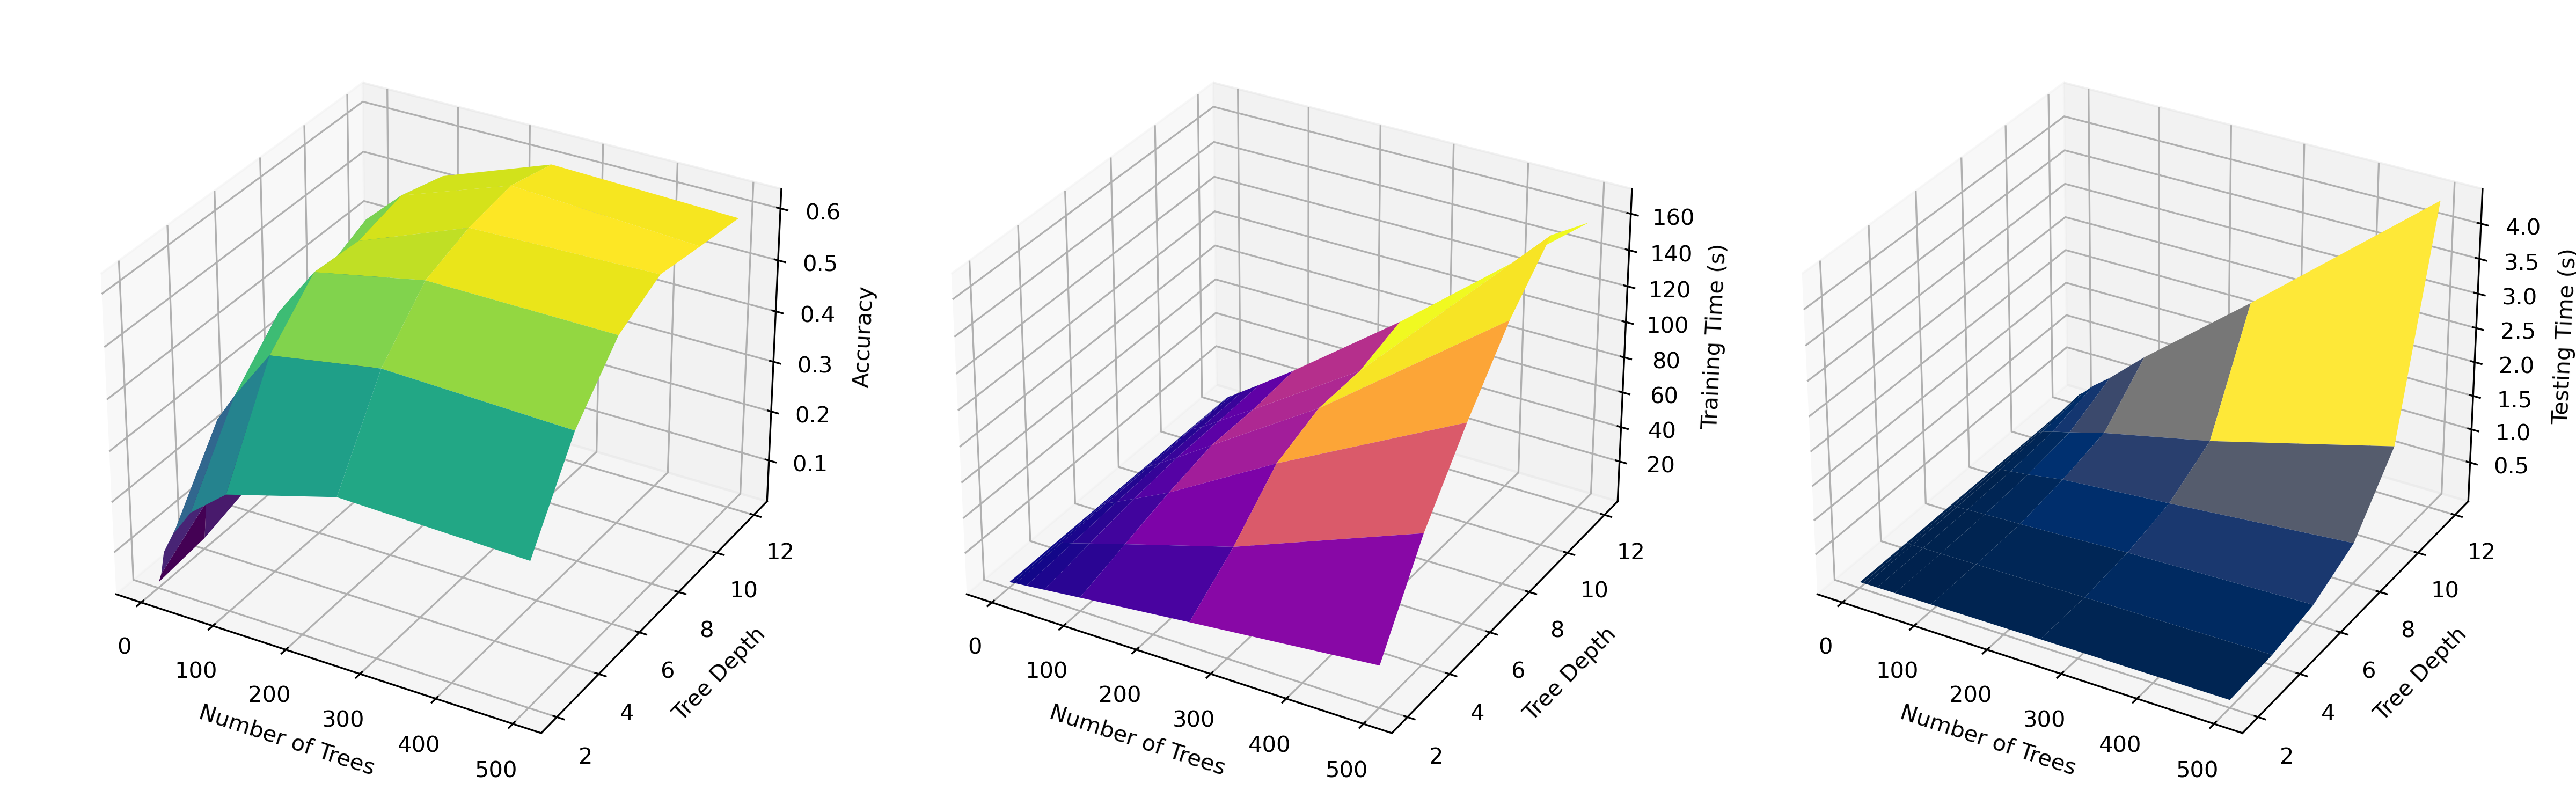
\includegraphics[width=\linewidth]{image/q5-fig1.png}
		\caption{Test accuracy, Training time, Testing time according to the number of tree and the depth of tree}
		\label{fig:q5-fig1}
	\end{subfigure}
	\begin{subfigure}[t]{\linewidth}
		\centering
		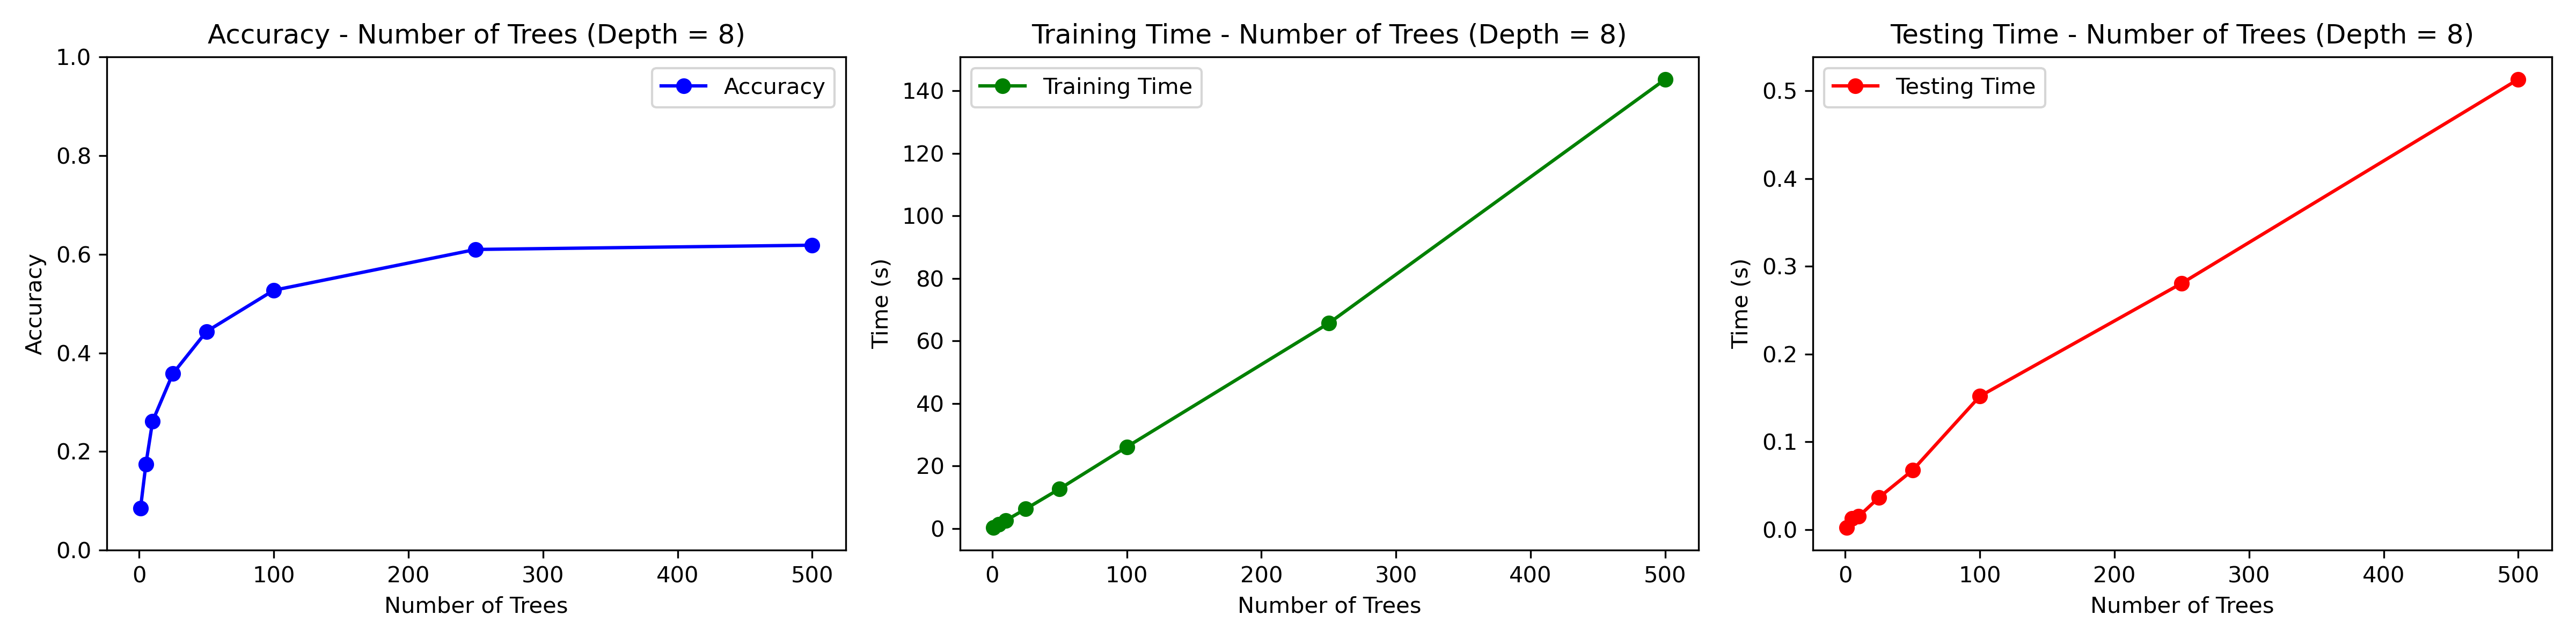
\includegraphics[width=\linewidth]{image/q5-fig2.png}
		\caption{Test accuracy, Training time, Testing time according to the number of tree (D = 8)}
		\label{fig:q5-fig2}
	\end{subfigure}
	\begin{subfigure}[t]{\linewidth}
		\centering
		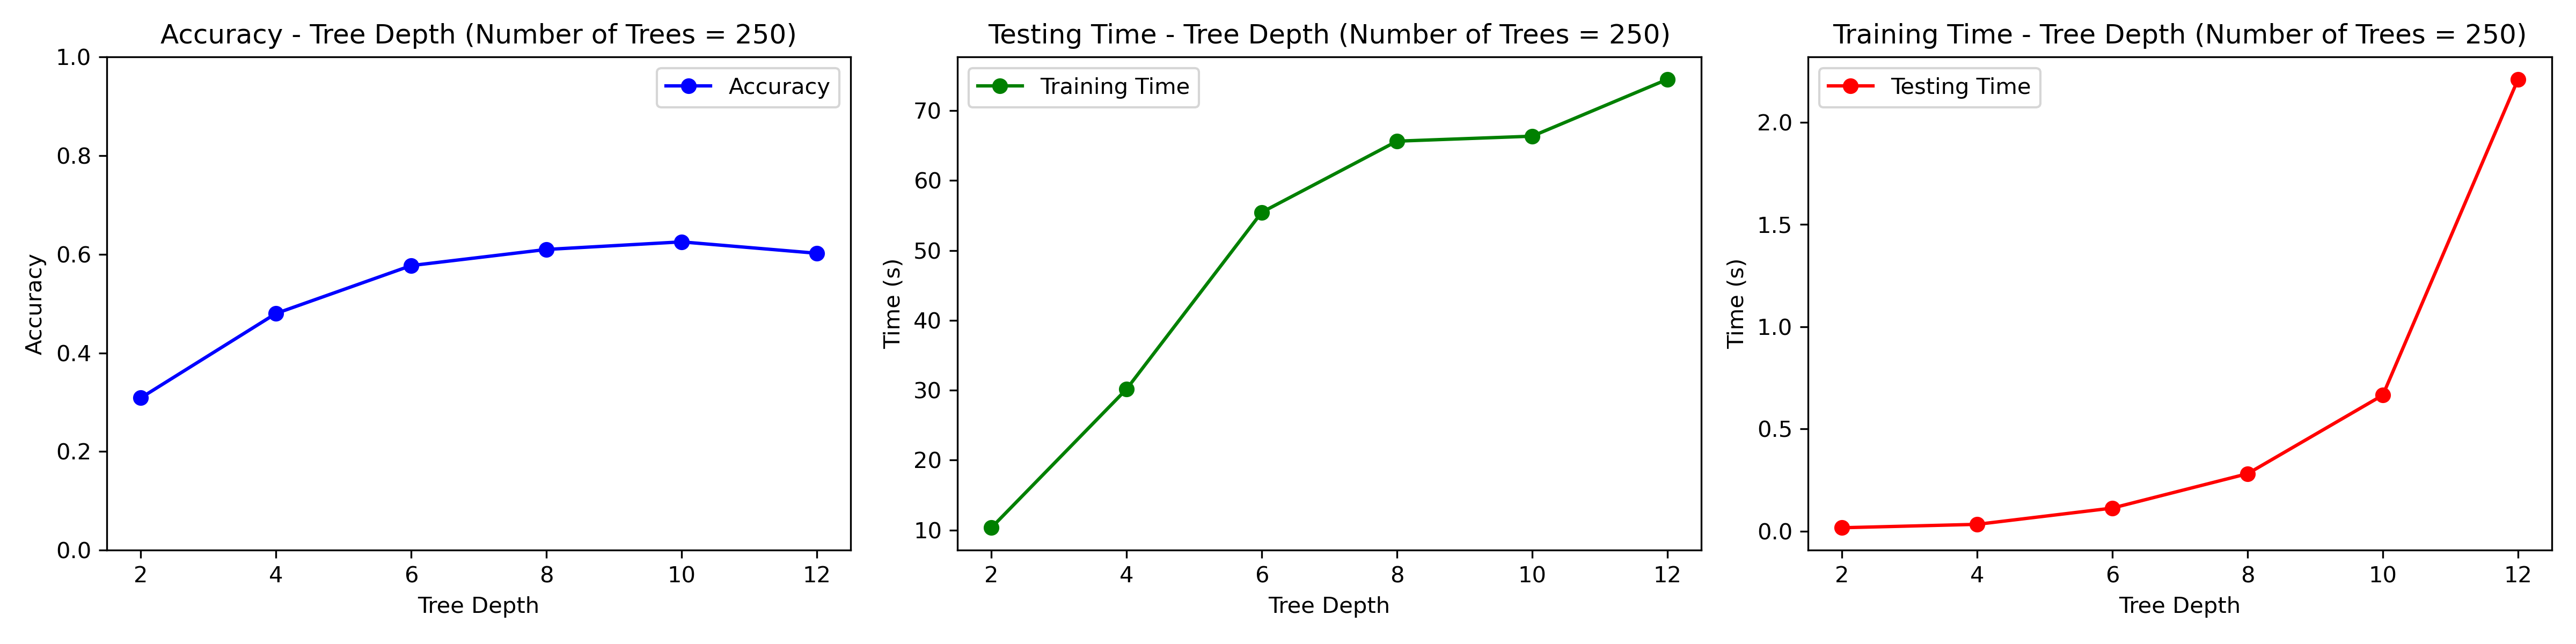
\includegraphics[width=\linewidth]{image/q5-fig3.png}
		\caption{Test accuracy, Training time, Testing time according to the depth of tree (N = 250)}
		\label{fig:q5-fig3}
	\end{subfigure}
	\caption{Test accuracy, training/testing time according to the number and depth of trees}
\end{figure}

\subsection{Randomness parameter}
Due to the high dimension image data, we randomly select dimensions and threshold values to create the split function. For each split function, we attempt $\rho$ random splits and choose the one with the highest information gain. There is a trade-off in the magnitude of $\rho$ value: If the $\rho$ value is too low, fewer splits are attempted, which reduces similarity between trees but increases the risk of the less-optimal split. Conversely, as $\rho$ increases, more various split functions are tested, leading to greater similarity among trees, which decreases the advantage of ensemble multiple trees. As shown in \cref{fig:q5-fig4}, accuracy initially increases with higher $\rho$ values until $\rho=10$ and then decreases, as expected. In \cref{fig:q5-fig5}, training time is same as expected, $O(\rho)$. However, since $\rho$ does not affect the resulting tree structure in training, it has constant testing time.

\begin{figure}[t]
	\centering
	\begin{subfigure}[t]{0.4\linewidth}
		\centering
		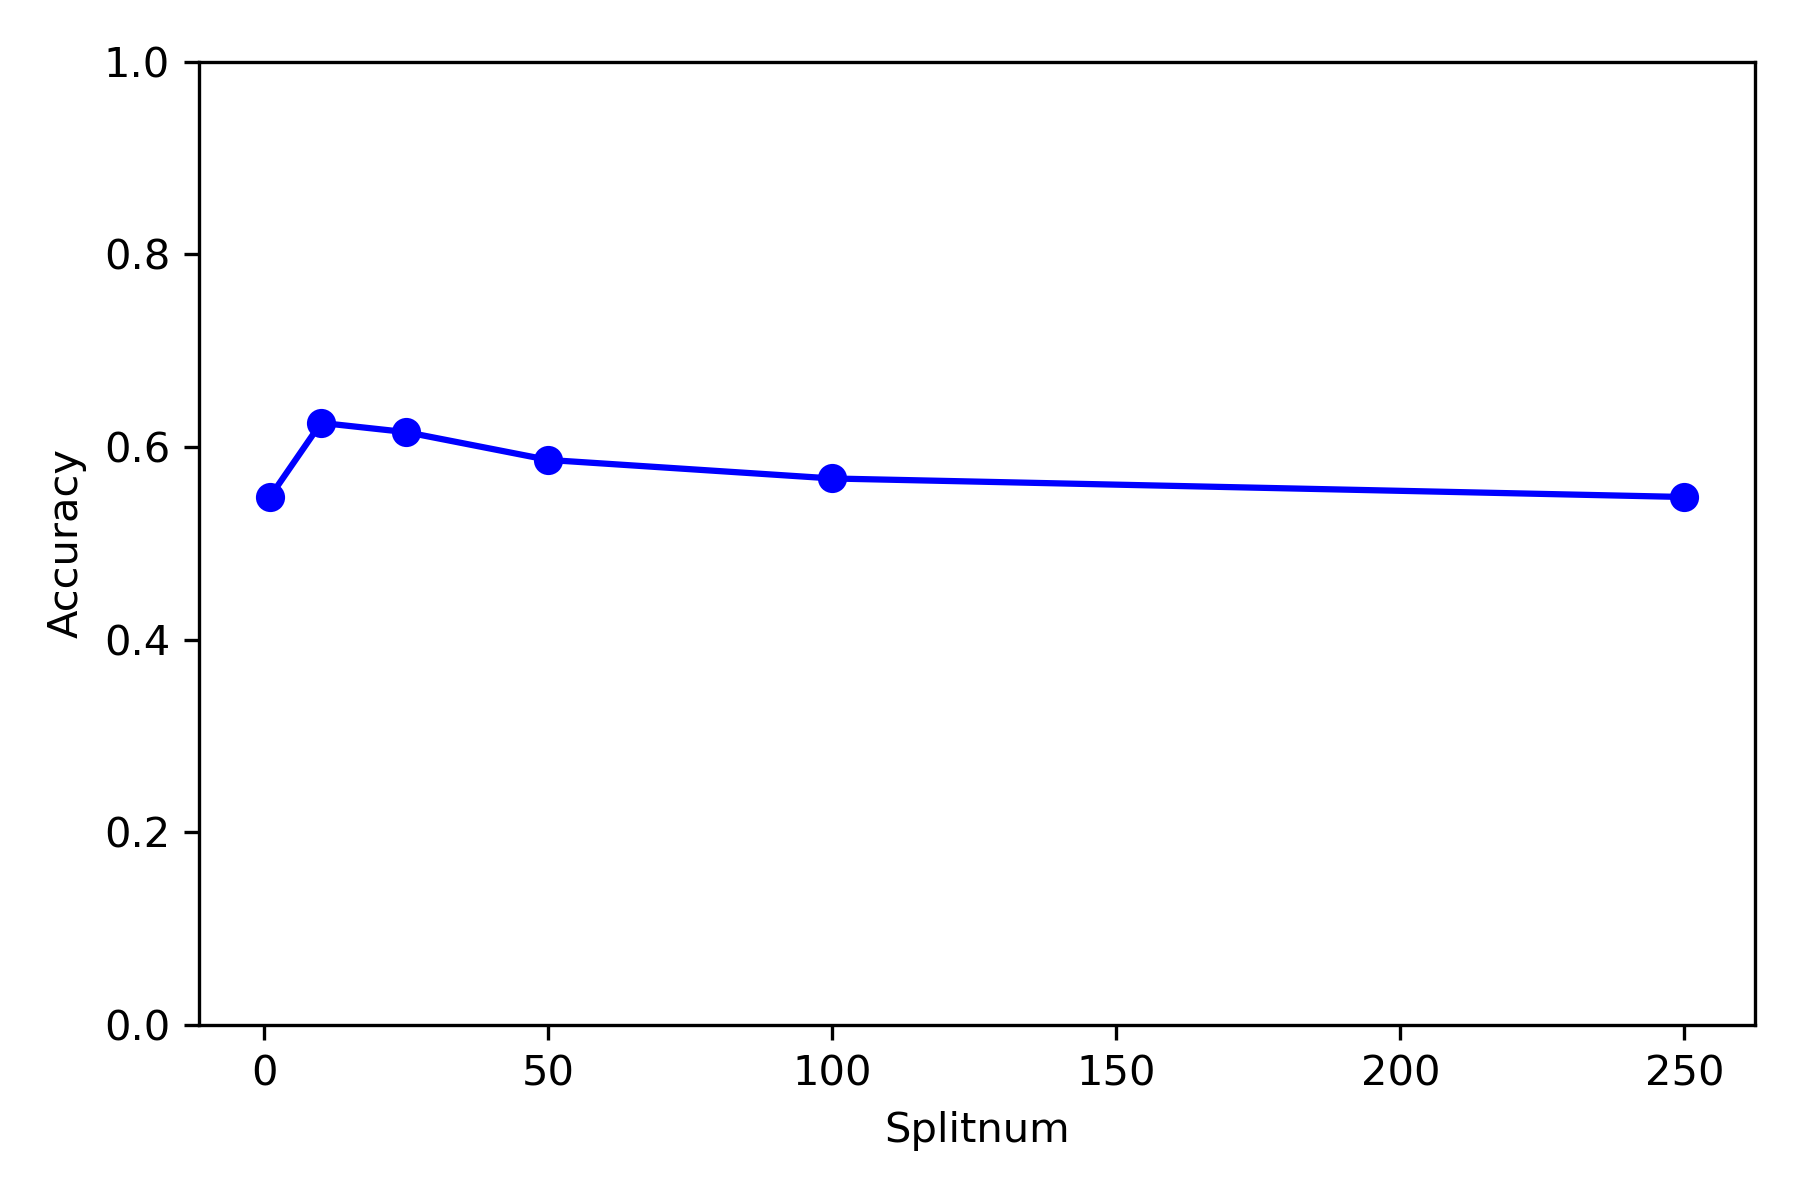
\includegraphics[width=\linewidth]{image/q5-fig4.png}
		\caption{Test accuracy according to the randomness parameter}
		\label{fig:q5-fig4}
	\end{subfigure}%
	\quad
	\begin{subfigure}[t]{0.4\linewidth}
		\centering
		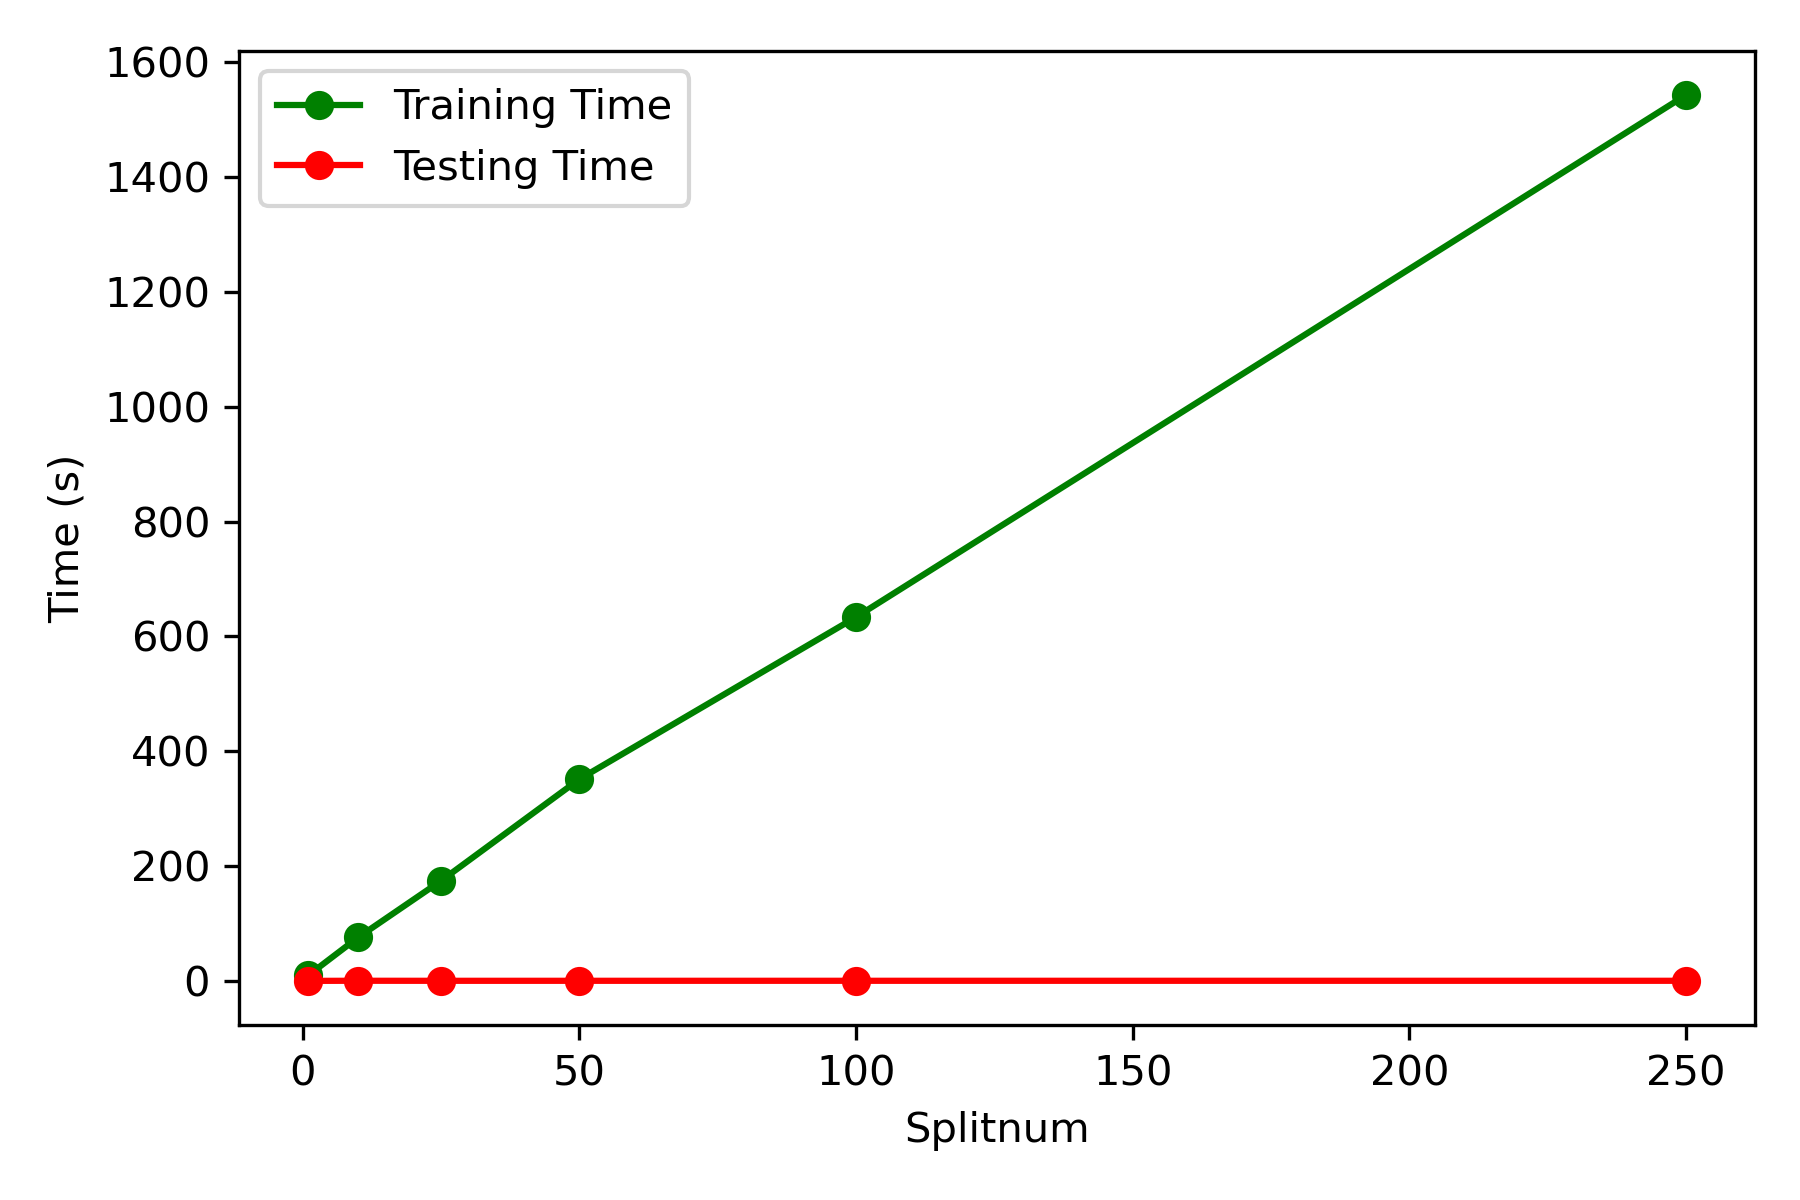
\includegraphics[width=\linewidth]{image/q5-fig5.png}
		\caption{Training time, Testing time according to the randomness parameter}
		\label{fig:q5-fig5}
	\end{subfigure}
	\caption{Test accuracy, training/testing time according to the randomness parameter}
\end{figure}

\subsection{Impact of the different types of weak-learners}
The impact of the weak learner are shown in \cref{fig:q5-fig7}. As expected, the axis-aligned method provides sufficiently good testing accuracy along with the shorter training and testing times. However, even with all other parameters being the same, the accuracy when using the two-pixel test is approximately 8.32\% higher. Therefore, the two-points test's information gain per split is greater than that of the axis-aligned method. Although other weak learners, such as linear and non-linear methods, were also implemented and tested, they took so long to measure training and testing times that it was expected impractical for real-time training/testing, and thus they were not included in the report.
\begin{figure}[t]
	\centering
	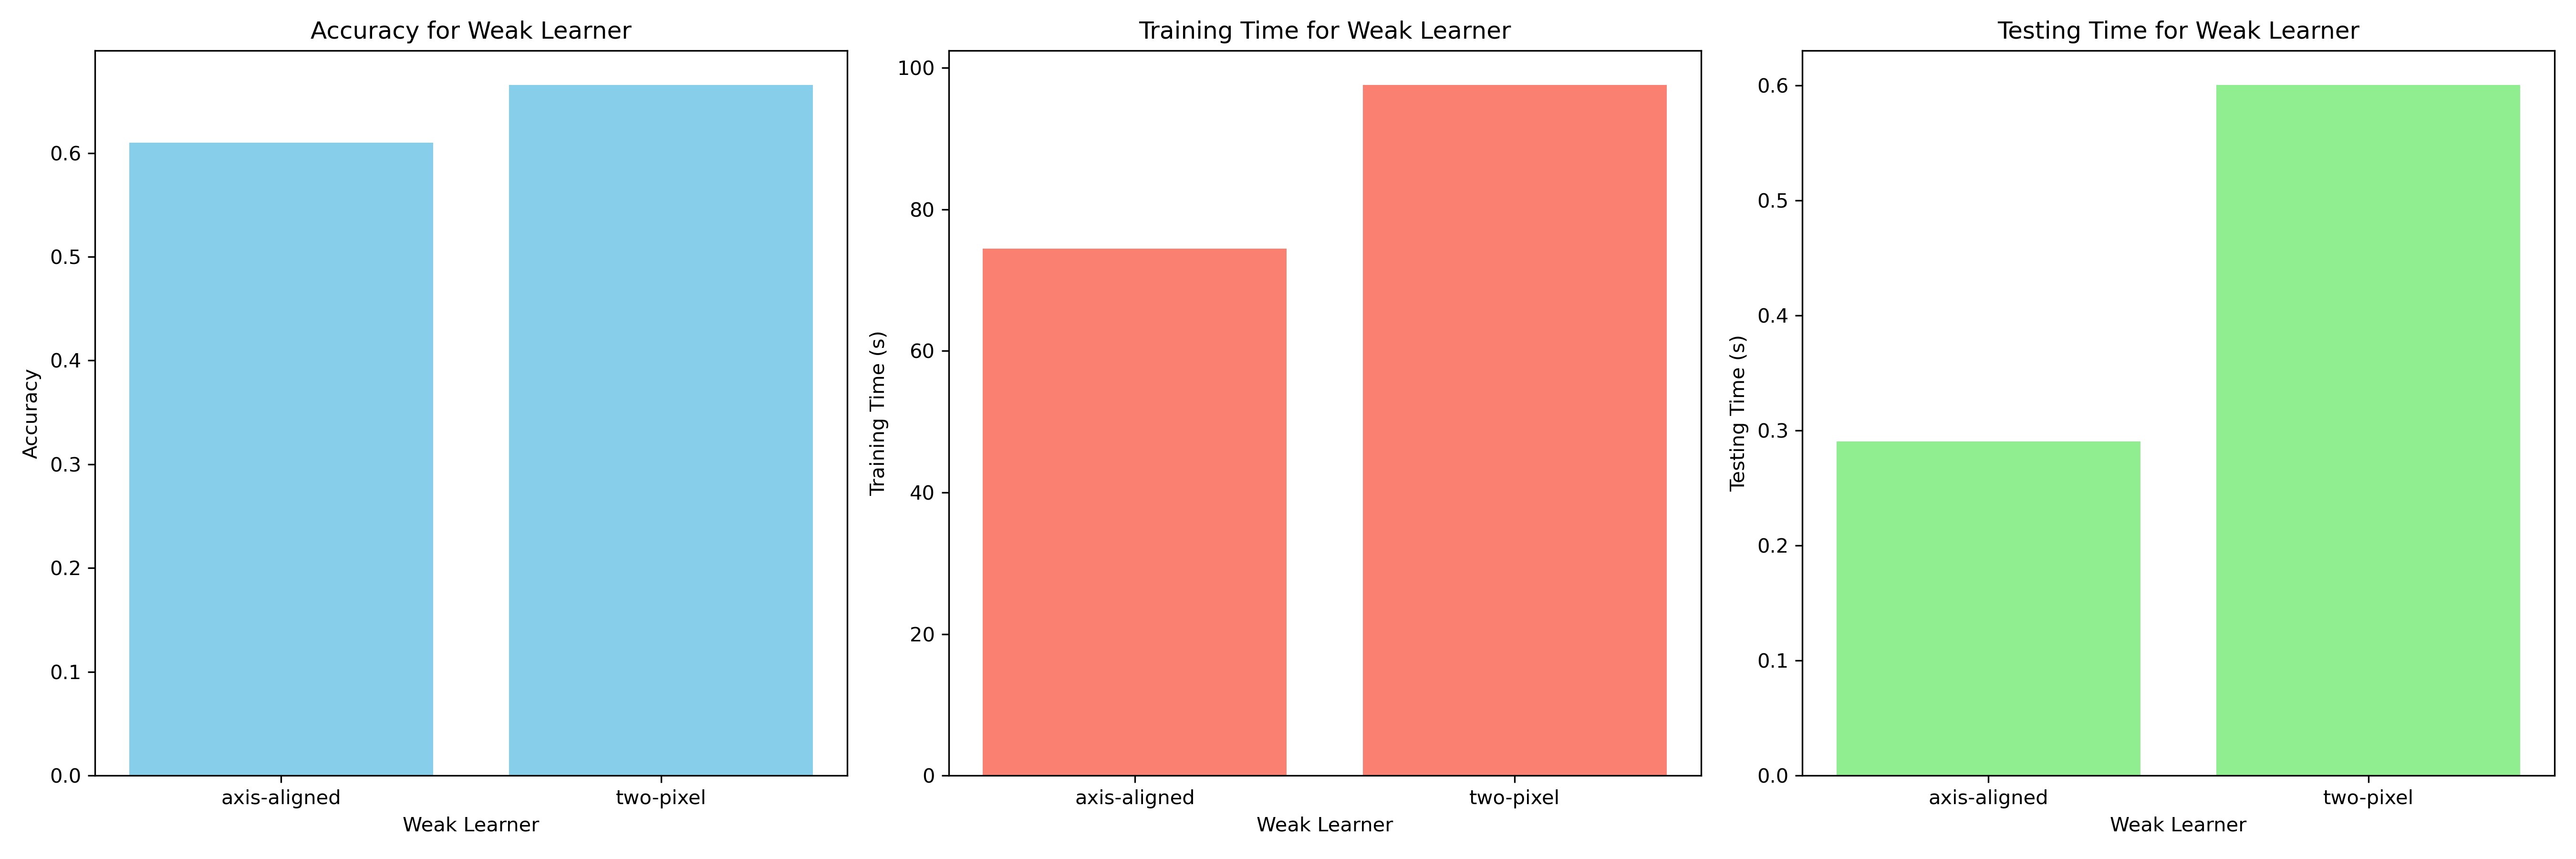
\includegraphics[width=0.8\linewidth]{image/q5-fig7.png}
	
	\caption{Axis-aligned vs Two-pixel test}
	\label{fig:q5-fig7}
\end{figure}


\subsection{Confusion matrix, Example success/failures, Information gain histogram}
The main results' confusion matrix, example success/failures, example node's histogram representing information gain along splitting are written in Appendix: \ref{subsec:Q5-1}, \ref{subsec:Q5-2}

\subsection{Comparision with PCA and PCA-LDA method}
Since parallel programming was not used our random forest, both the training and testing times are significantly large compared to the PCA and PCA-LDA methods. Because raw pixel values were used directly as inputs, the optimal accuracy of Q1 PCA is almost identical to random forest's result. Overall, the accuracy is much lower compared to the PCA-LDA method, indicating that in situations where the size of the training dataset is small ($N << D$), the random forest is relatively less suitable. Additionally, similar to the PCA-LDA ensemble, as the number of base models (~tree) increases, there is a tendency for accuracy to improve, indicating that the 'ensemble models' is beneficial.
